\documentclass[1p]{elsarticle_modified}
%\bibliographystyle{elsarticle-num}

%\usepackage[colorlinks]{hyperref}
%\usepackage{abbrmath_seonhwa} %\Abb, \Ascr, \Acal ,\Abf, \Afrak
\usepackage{amsfonts}
\usepackage{amssymb}
\usepackage{amsmath}
\usepackage{amsthm}
\usepackage{scalefnt}
\usepackage{amsbsy}
\usepackage{kotex}
\usepackage{caption}
\usepackage{subfig}
\usepackage{color}
\usepackage{graphicx}
\usepackage{xcolor} %% white, black, red, green, blue, cyan, magenta, yellow
\usepackage{float}
\usepackage{setspace}
\usepackage{hyperref}

\usepackage{tikz}
\usetikzlibrary{arrows}

\usepackage{multirow}
\usepackage{array} % fixed length table
\usepackage{hhline}

%%%%%%%%%%%%%%%%%%%%%
\makeatletter
\renewcommand*\env@matrix[1][\arraystretch]{%
	\edef\arraystretch{#1}%
	\hskip -\arraycolsep
	\let\@ifnextchar\new@ifnextchar
	\array{*\c@MaxMatrixCols c}}
\makeatother %https://tex.stackexchange.com/questions/14071/how-can-i-increase-the-line-spacing-in-a-matrix
%%%%%%%%%%%%%%%

\usepackage[normalem]{ulem}

\newcommand{\msout}[1]{\ifmmode\text{\sout{\ensuremath{#1}}}\else\sout{#1}\fi}
%SOURCE: \msout is \stkout macro in https://tex.stackexchange.com/questions/20609/strikeout-in-math-mode

\newcommand{\cancel}[1]{
	\ifmmode
	{\color{red}\msout{#1}}
	\else
	{\color{red}\sout{#1}}
	\fi
}

\newcommand{\add}[1]{
	{\color{blue}\uwave{#1}}
}

\newcommand{\replace}[2]{
	\ifmmode
	{\color{red}\msout{#1}}{\color{blue}\uwave{#2}}
	\else
	{\color{red}\sout{#1}}{\color{blue}\uwave{#2}}
	\fi
}

\newcommand{\Sol}{\mathcal{S}} %segment
\newcommand{\D}{D} %diagram
\newcommand{\A}{\mathcal{A}} %arc


%%%%%%%%%%%%%%%%%%%%%%%%%%%%%5 test

\def\sl{\operatorname{\textup{SL}}(2,\Cbb)}
\def\psl{\operatorname{\textup{PSL}}(2,\Cbb)}
\def\quan{\mkern 1mu \triangleright \mkern 1mu}

\theoremstyle{definition}
\newtheorem{thm}{Theorem}[section]
\newtheorem{prop}[thm]{Proposition}
\newtheorem{lem}[thm]{Lemma}
\newtheorem{ques}[thm]{Question}
\newtheorem{cor}[thm]{Corollary}
\newtheorem{defn}[thm]{Definition}
\newtheorem{exam}[thm]{Example}
\newtheorem{rmk}[thm]{Remark}
\newtheorem{alg}[thm]{Algorithm}

\newcommand{\I}{\sqrt{-1}}
\begin{document}

%\begin{frontmatter}
%
%\title{Boundary parabolic representations of knots up to 8 crossings}
%
%%% Group authors per affiliation:
%\author{Yunhi Cho} 
%\address{Department of Mathematics, University of Seoul, Seoul, Korea}
%\ead{yhcho@uos.ac.kr}
%
%
%\author{Seonhwa Kim} %\fnref{s_kim}}
%\address{Center for Geometry and Physics, Institute for Basic Science, Pohang, 37673, Korea}
%\ead{ryeona17@ibs.re.kr}
%
%\author{Hyuk Kim}
%\address{Department of Mathematical Sciences, Seoul National University, Seoul 08826, Korea}
%\ead{hyukkim@snu.ac.kr}
%
%\author{Seokbeom Yoon}
%\address{Department of Mathematical Sciences, Seoul National University, Seoul, 08826,  Korea}
%\ead{sbyoon15@snu.ac.kr}
%
%\begin{abstract}
%We find all boundary parabolic representation of knots up to 8 crossings.
%
%\end{abstract}
%\begin{keyword}
%    \MSC[2010] 57M25 
%\end{keyword}
%
%\end{frontmatter}

%\linenumbers
%\tableofcontents
%
\newcommand\colored[1]{\textcolor{white}{\rule[-0.35ex]{0.8em}{1.4ex}}\kern-0.8em\color{red} #1}%
%\newcommand\colored[1]{\textcolor{white}{ #1}\kern-2.17ex	\textcolor{white}{ #1}\kern-1.81ex	\textcolor{white}{ #1}\kern-2.15ex\color{red}#1	}

{\Large $\underline{12n_{0672}~(K12n_{0672})}$}

\setlength{\tabcolsep}{10pt}
\renewcommand{\arraystretch}{1.6}
\vspace{1cm}\begin{tabular}{m{100pt}>{\centering\arraybackslash}m{274pt}}
\multirow{5}{120pt}{
	\centering
	\includegraphics[width=112pt]{../../../GIT/diagram.site/Diagrams/png/2761_12n_0672.png}\\
\ \ \ A knot diagram\footnotemark}&
\allowdisplaybreaks
\textbf{Linearized knot diagam} \\
\cline{2-2}
 &
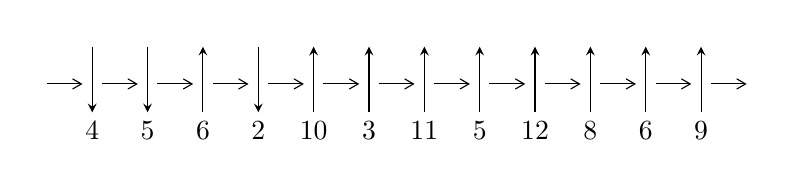
\begin{tikzpicture}[x=20pt, y=17pt]
	% nodes
	\node (C0) at (0, 0) {};
	\node (C1) at (1, 0) {};
	\node (C1U) at (1, +1) {};
	\node (C1D) at (1, -1) {4};

	\node (C2) at (2, 0) {};
	\node (C2U) at (2, +1) {};
	\node (C2D) at (2, -1) {5};

	\node (C3) at (3, 0) {};
	\node (C3U) at (3, +1) {};
	\node (C3D) at (3, -1) {6};

	\node (C4) at (4, 0) {};
	\node (C4U) at (4, +1) {};
	\node (C4D) at (4, -1) {2};

	\node (C5) at (5, 0) {};
	\node (C5U) at (5, +1) {};
	\node (C5D) at (5, -1) {10};

	\node (C6) at (6, 0) {};
	\node (C6U) at (6, +1) {};
	\node (C6D) at (6, -1) {3};

	\node (C7) at (7, 0) {};
	\node (C7U) at (7, +1) {};
	\node (C7D) at (7, -1) {11};

	\node (C8) at (8, 0) {};
	\node (C8U) at (8, +1) {};
	\node (C8D) at (8, -1) {5};

	\node (C9) at (9, 0) {};
	\node (C9U) at (9, +1) {};
	\node (C9D) at (9, -1) {12};

	\node (C10) at (10, 0) {};
	\node (C10U) at (10, +1) {};
	\node (C10D) at (10, -1) {8};

	\node (C11) at (11, 0) {};
	\node (C11U) at (11, +1) {};
	\node (C11D) at (11, -1) {6};

	\node (C12) at (12, 0) {};
	\node (C12U) at (12, +1) {};
	\node (C12D) at (12, -1) {9};
	\node (C13) at (13, 0) {};

	% arrows
	\draw[->,>={angle 60}]
	(C0) edge (C1) (C1) edge (C2) (C2) edge (C3) (C3) edge (C4) (C4) edge (C5) (C5) edge (C6) (C6) edge (C7) (C7) edge (C8) (C8) edge (C9) (C9) edge (C10) (C10) edge (C11) (C11) edge (C12) (C12) edge (C13) ;	\draw[->,>=stealth]
	(C1U) edge (C1D) (C2U) edge (C2D) (C3D) edge (C3U) (C4U) edge (C4D) (C5D) edge (C5U) (C6D) edge (C6U) (C7D) edge (C7U) (C8D) edge (C8U) (C9D) edge (C9U) (C10D) edge (C10U) (C11D) edge (C11U) (C12D) edge (C12U) ;
	\end{tikzpicture} \\
\hhline{~~} \\& 
\textbf{Solving Sequence} \\ \cline{2-2} 
 &
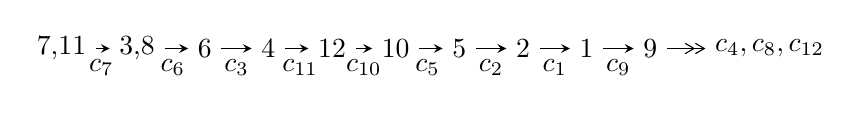
\begin{tikzpicture}[x=23pt, y=7pt]
	% node
	\node (A0) at (-1/8, 0) {7,11};
	\node (A1) at (17/16, 0) {3,8};
	\node (A2) at (17/8, 0) {6};
	\node (A3) at (25/8, 0) {4};
	\node (A4) at (33/8, 0) {12};
	\node (A5) at (41/8, 0) {10};
	\node (A6) at (49/8, 0) {5};
	\node (A7) at (57/8, 0) {2};
	\node (A8) at (65/8, 0) {1};
	\node (A9) at (73/8, 0) {9};
	\node (C1) at (1/2, -1) {$c_{7}$};
	\node (C2) at (13/8, -1) {$c_{6}$};
	\node (C3) at (21/8, -1) {$c_{3}$};
	\node (C4) at (29/8, -1) {$c_{11}$};
	\node (C5) at (37/8, -1) {$c_{10}$};
	\node (C6) at (45/8, -1) {$c_{5}$};
	\node (C7) at (53/8, -1) {$c_{2}$};
	\node (C8) at (61/8, -1) {$c_{1}$};
	\node (C9) at (69/8, -1) {$c_{9}$};
	\node (A10) at (11, 0) {$c_{4},c_{8},c_{12}$};

	% edge
	\draw[->,>=stealth]	
	(A0) edge (A1) (A1) edge (A2) (A2) edge (A3) (A3) edge (A4) (A4) edge (A5) (A5) edge (A6) (A6) edge (A7) (A7) edge (A8) (A8) edge (A9) ;
	\draw[->>,>={angle 60}]	
	(A9) edge (A10);
\end{tikzpicture} \\ 

\end{tabular} \\

\footnotetext{
The image of knot diagram is generated by the software ``\textbf{Draw programme}" developed by Andrew Bartholomew(\url{http://www.layer8.co.uk/maths/draw/index.htm\#Running-draw}), where we modified some parts for our purpose(\url{https://github.com/CATsTAILs/LinksPainter}).
}\phantom \\ \newline 
\centering \textbf{Ideals for irreducible components\footnotemark of $X_{\text{par}}$} 
 
\begin{align*}
I^u_{1}&=\langle 
140432815 u^{21}-8970077 u^{20}+\cdots+415372544 b-54946683,\\
\phantom{I^u_{1}}&\phantom{= \langle  }2854951501 u^{21}+303304377 u^{20}+\cdots+6645960704 a-7253385201,\;u^{22}+3 u^{20}+\cdots+u+1\rangle \\
I^u_{2}&=\langle 
-17272682156856 u^{19}+65400234558575 u^{18}+\cdots+646621574147963 b+203992951331482,\\
\phantom{I^u_{2}}&\phantom{= \langle  }3.50596\times10^{15} u^{19}-1.00606\times10^{16} u^{18}+\cdots+1.09926\times10^{16} a-4.23310\times10^{16},\;u^{20}-2 u^{19}+\cdots-4 u+17\rangle \\
I^u_{3}&=\langle 
b,\;-5 u^2+4 a+3 u-11,\;u^3+2 u+1\rangle \\
I^u_{4}&=\langle 
-243 a^4 u+1435 a^3 u+\cdots+487 a+424,\;a^5-4 a^4 u-5 a^4+9 a^3 u+2 a^3-6 a^2+6 a u+7 a- u,\;u^2+1\rangle \\
I^u_{5}&=\langle 
b,\;u^3+a+u,\;u^4- u^3+2 u^2-2 u+1\rangle \\
\\
\end{align*}
\raggedright * 5 irreducible components of $\dim_{\mathbb{C}}=0$, with total 59 representations.\\
\footnotetext{All coefficients of polynomials are rational numbers. But the coefficients are sometimes approximated in decimal forms when there is not enough margin.}
\newpage
\renewcommand{\arraystretch}{1}
\centering \section*{I. $I^u_{1}= \langle 1.40\times10^{8} u^{21}-8.97\times10^{6} u^{20}+\cdots+4.15\times10^{8} b-5.49\times10^{7},\;2.85\times10^{9} u^{21}+3.03\times10^{8} u^{20}+\cdots+6.65\times10^{9} a-7.25\times10^{9},\;u^{22}+3 u^{20}+\cdots+u+1 \rangle$}
\flushleft \textbf{(i) Arc colorings}\\
\begin{tabular}{m{7pt} m{180pt} m{7pt} m{180pt} }
\flushright $a_{7}=$&$\begin{pmatrix}1\\0\end{pmatrix}$ \\
\flushright $a_{11}=$&$\begin{pmatrix}0\\u\end{pmatrix}$ \\
\flushright $a_{3}=$&$\begin{pmatrix}-0.429577 u^{21}-0.0456374 u^{20}+\cdots-2.64683 u+1.09140\\-0.338089 u^{21}+0.0215953 u^{20}+\cdots-1.82898 u+0.132283\end{pmatrix}$ \\
\flushright $a_{8}=$&$\begin{pmatrix}1\\- u^2\end{pmatrix}$ \\
\flushright $a_{6}=$&$\begin{pmatrix}-0.339086 u^{21}-0.230329 u^{20}+\cdots-3.30702 u+0.269143\\0.141109 u^{21}-0.152381 u^{20}+\cdots-1.58891 u-0.881521\end{pmatrix}$ \\
\flushright $a_{4}=$&$\begin{pmatrix}0.119809 u^{21}-0.185566 u^{20}+\cdots-4.21378 u-0.352810\\-0.0118881 u^{21}+0.0634552 u^{20}+\cdots+1.25768 u+0.426641\end{pmatrix}$ \\
\flushright $a_{12}=$&$\begin{pmatrix}-0.00781250 u^{21}-0.00781250 u^{20}+\cdots-1.98438 u-0.992188\\0.0156250 u^{21}+0.0156250 u^{20}+\cdots+1.96875 u-0.0156250\end{pmatrix}$ \\
\flushright $a_{10}=$&$\begin{pmatrix}- u\\u^3+u\end{pmatrix}$ \\
\flushright $a_{5}=$&$\begin{pmatrix}-0.329484 u^{21}-0.213284 u^{20}+\cdots-3.71828 u-0.0429626\\0.169327 u^{21}-0.142245 u^{20}+\cdots-1.15100 u-0.552370\end{pmatrix}$ \\
\flushright $a_{2}=$&$\begin{pmatrix}0.371416 u^{21}+0.116662 u^{20}+\cdots-0.554103 u+0.690043\\-0.245528 u^{21}+0.287886 u^{20}+\cdots+0.564340 u+1.00801\end{pmatrix}$ \\
\flushright $a_{1}=$&$\begin{pmatrix}0.0156250 u^{21}+0.0156250 u^{20}+\cdots+1.96875 u+0.984375\\-0.0312500 u^{21}-0.0312500 u^{20}+\cdots-1.93750 u+0.0312500\end{pmatrix}$ \\
\flushright $a_{9}=$&$\begin{pmatrix}-0.00781250 u^{21}-0.00781250 u^{20}+\cdots-1.98438 u+0.00781250\\0.0156250 u^{21}+0.0156250 u^{20}+\cdots+0.968750 u-0.0156250\end{pmatrix}$\\&\end{tabular}
\flushleft \textbf{(ii) Obstruction class $= -1$}\\~\\
\flushleft \textbf{(iii) Cusp Shapes $= \frac{63242885225}{26583842816} u^{21}-\frac{275520283}{26583842816} u^{20}+\cdots-\frac{34653626479}{13291921408} u+\frac{128655382851}{26583842816}$}\\~\\
\newpage\renewcommand{\arraystretch}{1}
\flushleft \textbf{(iv) u-Polynomials at the component}\newline \\
\begin{tabular}{m{50pt}|m{274pt}}
Crossings & \hspace{64pt}u-Polynomials at each crossing \\
\hline $$\begin{aligned}c_{1},c_{2},c_{4}\end{aligned}$$&$\begin{aligned}
&u^{22}-4 u^{21}+\cdots+225 u-16
\end{aligned}$\\
\hline $$\begin{aligned}c_{3},c_{6}\end{aligned}$$&$\begin{aligned}
&u^{22}+3 u^{21}+\cdots-432 u+128
\end{aligned}$\\
\hline $$\begin{aligned}c_{5}\end{aligned}$$&$\begin{aligned}
&u^{22}+6 u^{21}+\cdots-12 u-4
\end{aligned}$\\
\hline $$\begin{aligned}c_{7},c_{9},c_{10}\\c_{12}\end{aligned}$$&$\begin{aligned}
&u^{22}+3 u^{20}+\cdots- u+1
\end{aligned}$\\
\hline $$\begin{aligned}c_{8},c_{11}\end{aligned}$$&$\begin{aligned}
&u^{22}-14 u^{20}+\cdots-160 u-32
\end{aligned}$\\
\hline
\end{tabular}\\~\\
\newpage\renewcommand{\arraystretch}{1}
\flushleft \textbf{(v) Riley Polynomials at the component}\newline \\
\begin{tabular}{m{50pt}|m{274pt}}
Crossings & \hspace{64pt}Riley Polynomials at each crossing \\
\hline $$\begin{aligned}c_{1},c_{2},c_{4}\end{aligned}$$&$\begin{aligned}
&y^{22}-12 y^{21}+\cdots-52961 y+256
\end{aligned}$\\
\hline $$\begin{aligned}c_{3},c_{6}\end{aligned}$$&$\begin{aligned}
&y^{22}-9 y^{21}+\cdots-181504 y+16384
\end{aligned}$\\
\hline $$\begin{aligned}c_{5}\end{aligned}$$&$\begin{aligned}
&y^{22}+4 y^{21}+\cdots-56 y+16
\end{aligned}$\\
\hline $$\begin{aligned}c_{7},c_{9},c_{10}\\c_{12}\end{aligned}$$&$\begin{aligned}
&y^{22}+6 y^{21}+\cdots+5 y+1
\end{aligned}$\\
\hline $$\begin{aligned}c_{8},c_{11}\end{aligned}$$&$\begin{aligned}
&y^{22}-28 y^{21}+\cdots-25600 y+1024
\end{aligned}$\\
\hline
\end{tabular}\\~\\
\newpage\flushleft \textbf{(vi) Complex Volumes and Cusp Shapes}
$$\begin{array}{c|c|c}  
\text{Solutions to }I^u_{1}& \I (\text{vol} + \sqrt{-1}CS) & \text{Cusp shape}\\
 \hline 
\begin{aligned}
u &= -0.928587 + 0.449929 I \\
a &= \phantom{-}0.444403 + 0.678322 I \\
b &= \phantom{-}0.105518 + 0.891648 I\end{aligned}
 & \phantom{-}0.73454 - 1.42308 I & \phantom{-}6.61226 - 1.84054 I \\ \hline\begin{aligned}
u &= -0.928587 - 0.449929 I \\
a &= \phantom{-}0.444403 - 0.678322 I \\
b &= \phantom{-}0.105518 - 0.891648 I\end{aligned}
 & \phantom{-}0.73454 + 1.42308 I & \phantom{-}6.61226 + 1.84054 I \\ \hline\begin{aligned}
u &= \phantom{-}0.805604 + 0.679539 I \\
a &= -0.675797 - 0.229153 I \\
b &= -0.10006 + 2.03537 I\end{aligned}
 & -0.58572 + 5.08842 I & \phantom{-}2.49387 - 7.97932 I \\ \hline\begin{aligned}
u &= \phantom{-}0.805604 - 0.679539 I \\
a &= -0.675797 + 0.229153 I \\
b &= -0.10006 - 2.03537 I\end{aligned}
 & -0.58572 - 5.08842 I & \phantom{-}2.49387 + 7.97932 I \\ \hline\begin{aligned}
u &= \phantom{-}0.016436 + 0.749464 I \\
a &= -0.280370 + 0.907991 I \\
b &= -0.438482 + 1.324440 I\end{aligned}
 & -8.18850 - 4.33155 I & \phantom{-}5.52961 + 2.50596 I \\ \hline\begin{aligned}
u &= \phantom{-}0.016436 - 0.749464 I \\
a &= -0.280370 - 0.907991 I \\
b &= -0.438482 - 1.324440 I\end{aligned}
 & -8.18850 + 4.33155 I & \phantom{-}5.52961 - 2.50596 I \\ \hline\begin{aligned}
u &= -0.722140\phantom{ +0.000000I} \\
a &= -3.32146\phantom{ +0.000000I} \\
b &= \phantom{-}0.476611\phantom{ +0.000000I}\end{aligned}
 & -0.565730\phantom{ +0.000000I} & \phantom{-}30.7730\phantom{ +0.000000I} \\ \hline\begin{aligned}
u &= \phantom{-}0.504021 + 0.445386 I \\
a &= \phantom{-}1.24386 - 0.98298 I \\
b &= -1.57016 + 0.27263 I\end{aligned}
 & -3.04188 + 1.34660 I & -0.20456 - 4.71267 I \\ \hline\begin{aligned}
u &= \phantom{-}0.504021 - 0.445386 I \\
a &= \phantom{-}1.24386 + 0.98298 I \\
b &= -1.57016 - 0.27263 I\end{aligned}
 & -3.04188 - 1.34660 I & -0.20456 + 4.71267 I \\ \hline\begin{aligned}
u &= \phantom{-}0.18886 + 1.40685 I \\
a &= \phantom{-}0.0573082 - 0.0995823 I \\
b &= -0.186722 - 0.594682 I\end{aligned}
 & -11.39190 + 5.29891 I & -11.9974 - 9.4087 I\\
 \hline 
 \end{array}$$\newpage$$\begin{array}{c|c|c}  
\text{Solutions to }I^u_{1}& \I (\text{vol} + \sqrt{-1}CS) & \text{Cusp shape}\\
 \hline 
\begin{aligned}
u &= \phantom{-}0.18886 - 1.40685 I \\
a &= \phantom{-}0.0573082 + 0.0995823 I \\
b &= -0.186722 + 0.594682 I\end{aligned}
 & -11.39190 - 5.29891 I & -11.9974 + 9.4087 I \\ \hline\begin{aligned}
u &= \phantom{-}1.05891 + 1.05062 I \\
a &= -1.049610 + 0.673117 I \\
b &= \phantom{-}2.15765 + 0.77847 I\end{aligned}
 & \phantom{-}6.65098 + 7.24014 I & \phantom{-}4.89876 - 5.30841 I \\ \hline\begin{aligned}
u &= \phantom{-}1.05891 - 1.05062 I \\
a &= -1.049610 - 0.673117 I \\
b &= \phantom{-}2.15765 - 0.77847 I\end{aligned}
 & \phantom{-}6.65098 - 7.24014 I & \phantom{-}4.89876 + 5.30841 I \\ \hline\begin{aligned}
u &= -0.82129 + 1.28483 I \\
a &= -0.697328 - 0.815294 I \\
b &= \phantom{-}1.43657 - 0.80726 I\end{aligned}
 & \phantom{-}4.44406 - 7.90966 I & \phantom{-}2.90985 + 4.71284 I \\ \hline\begin{aligned}
u &= -0.82129 - 1.28483 I \\
a &= -0.697328 + 0.815294 I \\
b &= \phantom{-}1.43657 + 0.80726 I\end{aligned}
 & \phantom{-}4.44406 + 7.90966 I & \phantom{-}2.90985 - 4.71284 I \\ \hline\begin{aligned}
u &= \phantom{-}0.072819 + 0.411896 I \\
a &= \phantom{-}1.38341 - 1.45349 I \\
b &= \phantom{-}0.042570 - 1.004680 I\end{aligned}
 & -1.51746 - 1.42204 I & \phantom{-}1.40403 + 3.03703 I \\ \hline\begin{aligned}
u &= \phantom{-}0.072819 - 0.411896 I \\
a &= \phantom{-}1.38341 + 1.45349 I \\
b &= \phantom{-}0.042570 + 1.004680 I\end{aligned}
 & -1.51746 + 1.42204 I & \phantom{-}1.40403 - 3.03703 I \\ \hline\begin{aligned}
u &= \phantom{-}0.87848 + 1.33285 I \\
a &= \phantom{-}0.999157 - 0.834434 I \\
b &= -1.68011 - 1.04071 I\end{aligned}
 & \phantom{-}3.8163 + 15.4146 I & \phantom{-}2.44451 - 7.76498 I \\ \hline\begin{aligned}
u &= \phantom{-}0.87848 - 1.33285 I \\
a &= \phantom{-}0.999157 + 0.834434 I \\
b &= -1.68011 + 1.04071 I\end{aligned}
 & \phantom{-}3.8163 - 15.4146 I & \phantom{-}2.44451 + 7.76498 I \\ \hline\begin{aligned}
u &= -1.22340 + 1.04887 I \\
a &= \phantom{-}0.809743 + 0.604171 I \\
b &= -1.63736 + 0.34201 I\end{aligned}
 & \phantom{-}6.54087 - 1.13702 I & \phantom{-}5.32063 - 0.78196 I\\
 \hline 
 \end{array}$$\newpage$$\begin{array}{c|c|c}  
\text{Solutions to }I^u_{1}& \I (\text{vol} + \sqrt{-1}CS) & \text{Cusp shape}\\
 \hline 
\begin{aligned}
u &= -1.22340 - 1.04887 I \\
a &= \phantom{-}0.809743 - 0.604171 I \\
b &= -1.63736 - 0.34201 I\end{aligned}
 & \phantom{-}6.54087 + 1.13702 I & \phantom{-}5.32063 + 0.78196 I \\ \hline\begin{aligned}
u &= -0.381582\phantom{ +0.000000I} \\
a &= \phantom{-}0.601919\phantom{ +0.000000I} \\
b &= \phantom{-}0.264566\phantom{ +0.000000I}\end{aligned}
 & \phantom{-}0.708401\phantom{ +0.000000I} & \phantom{-}14.4670\phantom{ +0.000000I}\\
 \hline 
 \end{array}$$\newpage\newpage\renewcommand{\arraystretch}{1}
\centering \section*{II. $I^u_{2}= \langle -1.73\times10^{13} u^{19}+6.54\times10^{13} u^{18}+\cdots+6.47\times10^{14} b+2.04\times10^{14},\;3.51\times10^{15} u^{19}-1.01\times10^{16} u^{18}+\cdots+1.10\times10^{16} a-4.23\times10^{16},\;u^{20}-2 u^{19}+\cdots-4 u+17 \rangle$}
\flushleft \textbf{(i) Arc colorings}\\
\begin{tabular}{m{7pt} m{180pt} m{7pt} m{180pt} }
\flushright $a_{7}=$&$\begin{pmatrix}1\\0\end{pmatrix}$ \\
\flushright $a_{11}=$&$\begin{pmatrix}0\\u\end{pmatrix}$ \\
\flushright $a_{3}=$&$\begin{pmatrix}-0.318939 u^{19}+0.915221 u^{18}+\cdots-12.9781 u+3.85087\\0.0267122 u^{19}-0.101141 u^{18}+\cdots+2.78094 u-0.315475\end{pmatrix}$ \\
\flushright $a_{8}=$&$\begin{pmatrix}1\\- u^2\end{pmatrix}$ \\
\flushright $a_{6}=$&$\begin{pmatrix}-0.103485 u^{19}+0.0740278 u^{18}+\cdots-8.11622 u+2.12405\\0.107851 u^{19}-0.263722 u^{18}+\cdots+3.65066 u-1.56320\end{pmatrix}$ \\
\flushright $a_{4}=$&$\begin{pmatrix}0.0148390 u^{19}+0.231650 u^{18}+\cdots-9.04018 u+5.85391\\0.0351704 u^{19}-0.0375853 u^{18}+\cdots+3.45642 u+0.00903128\end{pmatrix}$ \\
\flushright $a_{12}=$&$\begin{pmatrix}0.352319 u^{19}-1.31815 u^{18}+\cdots+3.33066 u-5.70075\\0.0984318 u^{19}-0.200644 u^{18}+\cdots+3.80209 u-1.16277\end{pmatrix}$ \\
\flushright $a_{10}=$&$\begin{pmatrix}- u\\u^3+u\end{pmatrix}$ \\
\flushright $a_{5}=$&$\begin{pmatrix}0.0188311 u^{19}-0.0566658 u^{18}+\cdots-6.85303 u+3.76850\\0.107524 u^{19}-0.232476 u^{18}+\cdots+4.01109 u-1.27070\end{pmatrix}$ \\
\flushright $a_{2}=$&$\begin{pmatrix}-0.104445 u^{19}+0.552187 u^{18}+\cdots-6.37772 u+4.35674\\-0.0495529 u^{19}+0.136649 u^{18}+\cdots+0.555470 u+0.796437\end{pmatrix}$ \\
\flushright $a_{1}=$&$\begin{pmatrix}-0.0250730 u^{19}+0.177714 u^{18}+\cdots-0.967992 u+3.13969\\-0.0256385 u^{19}+0.0848373 u^{18}+\cdots+0.0314805 u+0.0289650\end{pmatrix}$ \\
\flushright $a_{9}=$&$\begin{pmatrix}0.469648 u^{19}-0.562887 u^{18}+\cdots-7.03901 u+5.29851\\-0.00409626 u^{19}+0.110585 u^{18}+\cdots+3.78370 u+1.79742\end{pmatrix}$\\&\end{tabular}
\flushleft \textbf{(ii) Obstruction class $= -1$}\\~\\
\flushleft \textbf{(iii) Cusp Shapes $= -\frac{141694095517749}{646621574147963} u^{19}+\frac{11086941637505}{646621574147963} u^{18}+\cdots-\frac{4773664927135288}{646621574147963} u+\frac{1070128990714232}{646621574147963}$}\\~\\
\newpage\renewcommand{\arraystretch}{1}
\flushleft \textbf{(iv) u-Polynomials at the component}\newline \\
\begin{tabular}{m{50pt}|m{274pt}}
Crossings & \hspace{64pt}u-Polynomials at each crossing \\
\hline $$\begin{aligned}c_{1},c_{2},c_{4}\end{aligned}$$&$\begin{aligned}
&(u^{10}-3 u^9+4 u^8+u^7-6 u^6+6 u^5+u^4-2 u^3+3 u^2-2 u+1)^2
\end{aligned}$\\
\hline $$\begin{aligned}c_{3},c_{6}\end{aligned}$$&$\begin{aligned}
&(u^{10}+u^9-7 u^8-8 u^7+13 u^6+14 u^5-2 u^4+2 u^3+13 u^2+12 u+4)^2
\end{aligned}$\\
\hline $$\begin{aligned}c_{5}\end{aligned}$$&$\begin{aligned}
&(u^{10}-2 u^9+3 u^8-2 u^7+4 u^6-3 u^5+3 u^4+3 u^2- u+1)^2
\end{aligned}$\\
\hline $$\begin{aligned}c_{7},c_{9},c_{10}\\c_{12}\end{aligned}$$&$\begin{aligned}
&u^{20}+2 u^{19}+\cdots+4 u+17
\end{aligned}$\\
\hline $$\begin{aligned}c_{8},c_{11}\end{aligned}$$&$\begin{aligned}
&u^{20}-3 u^{18}+\cdots+35738 u+11449
\end{aligned}$\\
\hline
\end{tabular}\\~\\
\newpage\renewcommand{\arraystretch}{1}
\flushleft \textbf{(v) Riley Polynomials at the component}\newline \\
\begin{tabular}{m{50pt}|m{274pt}}
Crossings & \hspace{64pt}Riley Polynomials at each crossing \\
\hline $$\begin{aligned}c_{1},c_{2},c_{4}\end{aligned}$$&$\begin{aligned}
&(y^{10}- y^9+10 y^8-11 y^7+26 y^6-30 y^5+y^4+14 y^3+3 y^2+2 y+1)^2
\end{aligned}$\\
\hline $$\begin{aligned}c_{3},c_{6}\end{aligned}$$&$\begin{aligned}
&(y^{10}-15 y^9+\cdots-40 y+16)^{2}
\end{aligned}$\\
\hline $$\begin{aligned}c_{5}\end{aligned}$$&$\begin{aligned}
&(y^{10}+2 y^9+9 y^8+14 y^7+28 y^6+31 y^5+35 y^4+20 y^3+15 y^2+5 y+1)^{2}
\end{aligned}$\\
\hline $$\begin{aligned}c_{7},c_{9},c_{10}\\c_{12}\end{aligned}$$&$\begin{aligned}
&y^{20}+6 y^{19}+\cdots+4064 y+289
\end{aligned}$\\
\hline $$\begin{aligned}c_{8},c_{11}\end{aligned}$$&$\begin{aligned}
&y^{20}-6 y^{19}+\cdots+896868864 y+131079601
\end{aligned}$\\
\hline
\end{tabular}\\~\\
\newpage\flushleft \textbf{(vi) Complex Volumes and Cusp Shapes}
$$\begin{array}{c|c|c}  
\text{Solutions to }I^u_{2}& \I (\text{vol} + \sqrt{-1}CS) & \text{Cusp shape}\\
 \hline 
\begin{aligned}
u &= \phantom{-}0.155799 + 0.881795 I \\
a &= \phantom{-}3.18440 - 1.02398 I \\
b &= -0.413972 + 0.524496 I\end{aligned}
 & -5.18909 + 0.79591 I & -0.779599 + 0.811554 I \\ \hline\begin{aligned}
u &= \phantom{-}0.155799 - 0.881795 I \\
a &= \phantom{-}3.18440 + 1.02398 I \\
b &= -0.413972 - 0.524496 I\end{aligned}
 & -5.18909 - 0.79591 I & -0.779599 - 0.811554 I \\ \hline\begin{aligned}
u &= \phantom{-}0.074318 + 1.117810 I \\
a &= \phantom{-}3.33328 - 3.01725 I \\
b &= -0.413972 - 0.524496 I\end{aligned}
 & -5.18909 - 0.79591 I & -0.779599 - 0.811554 I \\ \hline\begin{aligned}
u &= \phantom{-}0.074318 - 1.117810 I \\
a &= \phantom{-}3.33328 + 3.01725 I \\
b &= -0.413972 + 0.524496 I\end{aligned}
 & -5.18909 + 0.79591 I & -0.779599 + 0.811554 I \\ \hline\begin{aligned}
u &= \phantom{-}0.922088 + 0.638802 I \\
a &= \phantom{-}0.862882 - 0.144749 I \\
b &= -0.793271 + 0.121626 I\end{aligned}
 & -3.70278 + 2.81207 I & \phantom{-}4.88002 - 4.64391 I \\ \hline\begin{aligned}
u &= \phantom{-}0.922088 - 0.638802 I \\
a &= \phantom{-}0.862882 + 0.144749 I \\
b &= -0.793271 - 0.121626 I\end{aligned}
 & -3.70278 - 2.81207 I & \phantom{-}4.88002 + 4.64391 I \\ \hline\begin{aligned}
u &= \phantom{-}0.027793 + 1.142750 I \\
a &= \phantom{-}0.806614 - 0.400008 I \\
b &= \phantom{-}0.620250 - 0.748934 I\end{aligned}
 & -2.14407 - 1.46073 I & \phantom{-}6.65931 + 3.28644 I \\ \hline\begin{aligned}
u &= \phantom{-}0.027793 - 1.142750 I \\
a &= \phantom{-}0.806614 + 0.400008 I \\
b &= \phantom{-}0.620250 + 0.748934 I\end{aligned}
 & -2.14407 + 1.46073 I & \phantom{-}6.65931 - 3.28644 I \\ \hline\begin{aligned}
u &= -1.218430 + 0.658057 I \\
a &= -0.880056 - 0.414251 I \\
b &= \phantom{-}1.96899 + 0.18613 I\end{aligned}
 & \phantom{-}6.57160 + 0.50253 I & \phantom{-}5.49701 + 0.08773 I \\ \hline\begin{aligned}
u &= -1.218430 - 0.658057 I \\
a &= -0.880056 + 0.414251 I \\
b &= \phantom{-}1.96899 - 0.18613 I\end{aligned}
 & \phantom{-}6.57160 - 0.50253 I & \phantom{-}5.49701 - 0.08773 I\\
 \hline 
 \end{array}$$\newpage$$\begin{array}{c|c|c}  
\text{Solutions to }I^u_{2}& \I (\text{vol} + \sqrt{-1}CS) & \text{Cusp shape}\\
 \hline 
\begin{aligned}
u &= \phantom{-}1.03744 + 1.07526 I \\
a &= -0.710678 + 0.832607 I \\
b &= \phantom{-}1.96899 + 0.18613 I\end{aligned}
 & \phantom{-}6.57160 + 0.50253 I & \phantom{-}5.49701 + 0.08773 I \\ \hline\begin{aligned}
u &= \phantom{-}1.03744 - 1.07526 I \\
a &= -0.710678 - 0.832607 I \\
b &= \phantom{-}1.96899 - 0.18613 I\end{aligned}
 & \phantom{-}6.57160 - 0.50253 I & \phantom{-}5.49701 - 0.08773 I \\ \hline\begin{aligned}
u &= \phantom{-}1.37291 + 0.66267 I \\
a &= \phantom{-}0.885501 - 0.517371 I \\
b &= -1.88200 + 0.46774 I\end{aligned}
 & \phantom{-}6.10927 - 7.40677 I & \phantom{-}4.74326 + 4.41038 I \\ \hline\begin{aligned}
u &= \phantom{-}1.37291 - 0.66267 I \\
a &= \phantom{-}0.885501 + 0.517371 I \\
b &= -1.88200 - 0.46774 I\end{aligned}
 & \phantom{-}6.10927 + 7.40677 I & \phantom{-}4.74326 - 4.41038 I \\ \hline\begin{aligned}
u &= -0.09604 + 1.52972 I \\
a &= -0.0133270 - 0.1369840 I \\
b &= -0.793271 - 0.121626 I\end{aligned}
 & -3.70278 - 2.81207 I & \phantom{-}4.88002 + 4.64391 I \\ \hline\begin{aligned}
u &= -0.09604 - 1.52972 I \\
a &= -0.0133270 + 0.1369840 I \\
b &= -0.793271 + 0.121626 I\end{aligned}
 & -3.70278 + 2.81207 I & \phantom{-}4.88002 - 4.64391 I \\ \hline\begin{aligned}
u &= -0.138308 + 0.379907 I \\
a &= -2.22932 - 2.47499 I \\
b &= \phantom{-}0.620250 + 0.748934 I\end{aligned}
 & -2.14407 + 1.46073 I & \phantom{-}6.65931 - 3.28644 I \\ \hline\begin{aligned}
u &= -0.138308 - 0.379907 I \\
a &= -2.22932 + 2.47499 I \\
b &= \phantom{-}0.620250 - 0.748934 I\end{aligned}
 & -2.14407 - 1.46073 I & \phantom{-}6.65931 + 3.28644 I \\ \hline\begin{aligned}
u &= -1.13757 + 1.18122 I \\
a &= \phantom{-}0.848938 + 0.551739 I \\
b &= -1.88200 + 0.46774 I\end{aligned}
 & \phantom{-}6.10927 - 7.40677 I & \phantom{-}4.74326 + 4.41038 I \\ \hline\begin{aligned}
u &= -1.13757 - 1.18122 I \\
a &= \phantom{-}0.848938 - 0.551739 I \\
b &= -1.88200 - 0.46774 I\end{aligned}
 & \phantom{-}6.10927 + 7.40677 I & \phantom{-}4.74326 - 4.41038 I\\
 \hline 
 \end{array}$$\newpage\newpage\renewcommand{\arraystretch}{1}
\centering \section*{III. $I^u_{3}= \langle b,\;-5 u^2+4 a+3 u-11,\;u^3+2 u+1 \rangle$}
\flushleft \textbf{(i) Arc colorings}\\
\begin{tabular}{m{7pt} m{180pt} m{7pt} m{180pt} }
\flushright $a_{7}=$&$\begin{pmatrix}1\\0\end{pmatrix}$ \\
\flushright $a_{11}=$&$\begin{pmatrix}0\\u\end{pmatrix}$ \\
\flushright $a_{3}=$&$\begin{pmatrix}\frac{5}{4} u^2-\frac{3}{4} u+\frac{11}{4}\\0\end{pmatrix}$ \\
\flushright $a_{8}=$&$\begin{pmatrix}1\\- u^2\end{pmatrix}$ \\
\flushright $a_{6}=$&$\begin{pmatrix}1\\0\end{pmatrix}$ \\
\flushright $a_{4}=$&$\begin{pmatrix}\frac{5}{4} u^2-\frac{3}{4} u+\frac{11}{4}\\0\end{pmatrix}$ \\
\flushright $a_{12}=$&$\begin{pmatrix}u\\u\end{pmatrix}$ \\
\flushright $a_{10}=$&$\begin{pmatrix}- u\\- u-1\end{pmatrix}$ \\
\flushright $a_{5}=$&$\begin{pmatrix}u^2+u+1\\u^2+2 u+1\end{pmatrix}$ \\
\flushright $a_{2}=$&$\begin{pmatrix}\frac{1}{4} u^2-\frac{7}{4} u+\frac{7}{4}\\- u^2-2 u-1\end{pmatrix}$ \\
\flushright $a_{1}=$&$\begin{pmatrix}- u^2- u-1\\- u^2-2 u-1\end{pmatrix}$ \\
\flushright $a_{9}=$&$\begin{pmatrix}u^2- u\\u^2- u-1\end{pmatrix}$\\&\end{tabular}
\flushleft \textbf{(ii) Obstruction class $= 1$}\\~\\
\flushleft \textbf{(iii) Cusp Shapes $= -\frac{69}{16} u^2+\frac{47}{16} u-\frac{7}{16}$}\\~\\
\newpage\renewcommand{\arraystretch}{1}
\flushleft \textbf{(iv) u-Polynomials at the component}\newline \\
\begin{tabular}{m{50pt}|m{274pt}}
Crossings & \hspace{64pt}u-Polynomials at each crossing \\
\hline $$\begin{aligned}c_{1},c_{2}\end{aligned}$$&$\begin{aligned}
&(u-1)^3
\end{aligned}$\\
\hline $$\begin{aligned}c_{3},c_{6}\end{aligned}$$&$\begin{aligned}
&u^3
\end{aligned}$\\
\hline $$\begin{aligned}c_{4}\end{aligned}$$&$\begin{aligned}
&(u+1)^3
\end{aligned}$\\
\hline $$\begin{aligned}c_{5}\end{aligned}$$&$\begin{aligned}
&u^3+3 u^2+5 u+2
\end{aligned}$\\
\hline $$\begin{aligned}c_{7},c_{9}\end{aligned}$$&$\begin{aligned}
&u^3+2 u+1
\end{aligned}$\\
\hline $$\begin{aligned}c_{8},c_{10},c_{11}\\c_{12}\end{aligned}$$&$\begin{aligned}
&u^3+2 u-1
\end{aligned}$\\
\hline
\end{tabular}\\~\\
\newpage\renewcommand{\arraystretch}{1}
\flushleft \textbf{(v) Riley Polynomials at the component}\newline \\
\begin{tabular}{m{50pt}|m{274pt}}
Crossings & \hspace{64pt}Riley Polynomials at each crossing \\
\hline $$\begin{aligned}c_{1},c_{2},c_{4}\end{aligned}$$&$\begin{aligned}
&(y-1)^3
\end{aligned}$\\
\hline $$\begin{aligned}c_{3},c_{6}\end{aligned}$$&$\begin{aligned}
&y^3
\end{aligned}$\\
\hline $$\begin{aligned}c_{5}\end{aligned}$$&$\begin{aligned}
&y^3+y^2+13 y-4
\end{aligned}$\\
\hline $$\begin{aligned}c_{7},c_{8},c_{9}\\c_{10},c_{11},c_{12}\end{aligned}$$&$\begin{aligned}
&y^3+4 y^2+4 y-1
\end{aligned}$\\
\hline
\end{tabular}\\~\\
\newpage\flushleft \textbf{(vi) Complex Volumes and Cusp Shapes}
$$\begin{array}{c|c|c}  
\text{Solutions to }I^u_{3}& \I (\text{vol} + \sqrt{-1}CS) & \text{Cusp shape}\\
 \hline 
\begin{aligned}
u &= \phantom{-}0.22670 + 1.46771 I \\
a &= -0.048505 - 0.268962 I \\
b &= \phantom{-0.000000 } 0\end{aligned}
 & -11.08570 + 5.13794 I & \phantom{-}9.29669 + 1.44162 I \\ \hline\begin{aligned}
u &= \phantom{-}0.22670 - 1.46771 I \\
a &= -0.048505 + 0.268962 I \\
b &= \phantom{-0.000000 } 0\end{aligned}
 & -11.08570 - 5.13794 I & \phantom{-}9.29669 - 1.44162 I \\ \hline\begin{aligned}
u &= -0.453398\phantom{ +0.000000I} \\
a &= \phantom{-}3.34701\phantom{ +0.000000I} \\
b &= \phantom{-0.000000 } 0\end{aligned}
 & -0.857735\phantom{ +0.000000I} & -2.65590\phantom{ +0.000000I}\\
 \hline 
 \end{array}$$\newpage\newpage\renewcommand{\arraystretch}{1}
\centering \section*{IV. $I^u_{4}= \langle -243 a^4 u+1435 a^3 u+\cdots+487 a+424,\;-4 a^4 u+9 a^3 u+\cdots-6 a^2+7 a,\;u^2+1 \rangle$}
\flushleft \textbf{(i) Arc colorings}\\
\begin{tabular}{m{7pt} m{180pt} m{7pt} m{180pt} }
\flushright $a_{7}=$&$\begin{pmatrix}1\\0\end{pmatrix}$ \\
\flushright $a_{11}=$&$\begin{pmatrix}0\\u\end{pmatrix}$ \\
\flushright $a_{3}=$&$\begin{pmatrix}a\\0.335172 a^{4} u-1.97931 a^{3} u+\cdots-0.671724 a-0.584828\end{pmatrix}$ \\
\flushright $a_{8}=$&$\begin{pmatrix}1\\1\end{pmatrix}$ \\
\flushright $a_{6}=$&$\begin{pmatrix}0.104828 a^{4} u+0.179310 a^{3} u+\cdots+0.711724 a+0.664828\\-0.00275862 a^{4} u+0.668966 a^{3} u+\cdots+0.307586 a-1.32276\end{pmatrix}$ \\
\flushright $a_{4}=$&$\begin{pmatrix}0.377931 a^{4} u-1.84828 a^{3} u+\cdots+0.0606897 a-0.582069\\0.0124138 a^{4} u-0.710345 a^{3} u+\cdots-1.68414 a+1.65241\end{pmatrix}$ \\
\flushright $a_{12}=$&$\begin{pmatrix}-0.397241 a^{4} u+1.93103 a^{3} u+\cdots+2.69241 a-0.0772414\\1\end{pmatrix}$ \\
\flushright $a_{10}=$&$\begin{pmatrix}- u\\0\end{pmatrix}$ \\
\flushright $a_{5}=$&$\begin{pmatrix}0.102069 a^{4} u+0.848276 a^{3} u+\cdots+1.01931 a-0.657931\\-0.00275862 a^{4} u+0.668966 a^{3} u+\cdots+0.307586 a-1.32276\end{pmatrix}$ \\
\flushright $a_{2}=$&$\begin{pmatrix}-0.263448 a^{4} u+1.78621 a^{3} u+\cdots+0.474483 a-0.223448\\0.131034 a^{4} u+0.324138 a^{3} u+\cdots+1.28966 a-2.26897\end{pmatrix}$ \\
\flushright $a_{1}=$&$\begin{pmatrix}-1\\0\end{pmatrix}$ \\
\flushright $a_{9}=$&$\begin{pmatrix}0.0468966 a^{4} u+0.827586 a^{3} u+\cdots+2.57103 a+0.286897\\- u\end{pmatrix}$\\&\end{tabular}
\flushleft \textbf{(ii) Obstruction class $= 1$}\\~\\
\flushleft \textbf{(iii) Cusp Shapes $= -\frac{28}{725} a^4 u-\frac{104}{725} a^4+\frac{24}{145} a^3 u+\frac{172}{145} a^3+\frac{48}{725} a^2 u-\frac{3136}{725} a^2-\frac{1156}{725} a u+\frac{3992}{725} a+\frac{2308}{725} u-\frac{3856}{725}$}\\~\\
\newpage\renewcommand{\arraystretch}{1}
\flushleft \textbf{(iv) u-Polynomials at the component}\newline \\
\begin{tabular}{m{50pt}|m{274pt}}
Crossings & \hspace{64pt}u-Polynomials at each crossing \\
\hline $$\begin{aligned}c_{1},c_{2}\end{aligned}$$&$\begin{aligned}
&(u^5+u^4-2 u^3- u^2+u-1)^2
\end{aligned}$\\
\hline $$\begin{aligned}c_{3}\end{aligned}$$&$\begin{aligned}
&(u^5- u^4+2 u^3- u^2+u-1)^2
\end{aligned}$\\
\hline $$\begin{aligned}c_{4}\end{aligned}$$&$\begin{aligned}
&(u^5- u^4-2 u^3+u^2+u+1)^2
\end{aligned}$\\
\hline $$\begin{aligned}c_{5}\end{aligned}$$&$\begin{aligned}
&u^{10}+u^8+8 u^6+3 u^4+3 u^2+1
\end{aligned}$\\
\hline $$\begin{aligned}c_{6}\end{aligned}$$&$\begin{aligned}
&(u^5+u^4+2 u^3+u^2+u+1)^2
\end{aligned}$\\
\hline $$\begin{aligned}c_{7},c_{9},c_{10}\\c_{12}\end{aligned}$$&$\begin{aligned}
&(u^2+1)^5
\end{aligned}$\\
\hline $$\begin{aligned}c_{8}\end{aligned}$$&$\begin{aligned}
&u^{10}+2 u^9+\cdots+96 u+32
\end{aligned}$\\
\hline $$\begin{aligned}c_{11}\end{aligned}$$&$\begin{aligned}
&u^{10}-2 u^9+\cdots-96 u+32
\end{aligned}$\\
\hline
\end{tabular}\\~\\
\newpage\renewcommand{\arraystretch}{1}
\flushleft \textbf{(v) Riley Polynomials at the component}\newline \\
\begin{tabular}{m{50pt}|m{274pt}}
Crossings & \hspace{64pt}Riley Polynomials at each crossing \\
\hline $$\begin{aligned}c_{1},c_{2},c_{4}\end{aligned}$$&$\begin{aligned}
&(y^5-5 y^4+8 y^3-3 y^2- y-1)^2
\end{aligned}$\\
\hline $$\begin{aligned}c_{3},c_{6}\end{aligned}$$&$\begin{aligned}
&(y^5+3 y^4+4 y^3+y^2- y-1)^2
\end{aligned}$\\
\hline $$\begin{aligned}c_{5}\end{aligned}$$&$\begin{aligned}
&(y^5+y^4+8 y^3+3 y^2+3 y+1)^2
\end{aligned}$\\
\hline $$\begin{aligned}c_{7},c_{9},c_{10}\\c_{12}\end{aligned}$$&$\begin{aligned}
&(y+1)^{10}
\end{aligned}$\\
\hline $$\begin{aligned}c_{8},c_{11}\end{aligned}$$&$\begin{aligned}
&y^{10}+12 y^8-592 y^6+4096 y^4-3840 y^2+1024
\end{aligned}$\\
\hline
\end{tabular}\\~\\
\newpage\flushleft \textbf{(vi) Complex Volumes and Cusp Shapes}
$$\begin{array}{c|c|c}  
\text{Solutions to }I^u_{4}& \I (\text{vol} + \sqrt{-1}CS) & \text{Cusp shape}\\
 \hline 
\begin{aligned}
u &= \phantom{-0.000000 -}1.000000 I \\
a &= -0.361438 - 0.927855 I \\
b &= -0.455697 - 1.200150 I\end{aligned}
 & -9.16243 + 4.40083 I & -4.74431 - 3.49859 I \\ \hline\begin{aligned}
u &= \phantom{-0.000000 -}1.000000 I \\
a &= \phantom{-}0.331455 + 0.820551 I \\
b &= \phantom{-}0.339110 - 0.822375 I\end{aligned}
 & -3.61897 - 1.53058 I & -0.51511 + 4.43065 I \\ \hline\begin{aligned}
u &= \phantom{-0.000000 -}1.000000 I \\
a &= \phantom{-}0.0768928 + 0.0902877 I \\
b &= -0.455697 + 1.200150 I\end{aligned}
 & -9.16243 - 4.40083 I & -4.74431 + 3.49859 I \\ \hline\begin{aligned}
u &= \phantom{-0.000000 -}1.000000 I \\
a &= \phantom{-}1.43128 + 1.79928 I \\
b &= \phantom{-}0.339110 + 0.822375 I\end{aligned}
 & -3.61897 + 1.53058 I & -0.51511 - 4.43065 I \\ \hline\begin{aligned}
u &= \phantom{-0.000000 -}1.000000 I \\
a &= \phantom{-}3.52181 + 2.21774 I \\
b &= -0.766826\phantom{ +0.000000I}\end{aligned}
 & -5.69095\phantom{ +0.000000I} & -1.48114 + 0. I\phantom{ +0.000000I} \\ \hline\begin{aligned}
u &= \phantom{-0.000000 } -1.000000 I \\
a &= -0.361438 + 0.927855 I \\
b &= -0.455697 + 1.200150 I\end{aligned}
 & -9.16243 - 4.40083 I & -4.74431 + 3.49859 I \\ \hline\begin{aligned}
u &= \phantom{-0.000000 } -1.000000 I \\
a &= \phantom{-}0.331455 - 0.820551 I \\
b &= \phantom{-}0.339110 + 0.822375 I\end{aligned}
 & -3.61897 + 1.53058 I & -0.51511 - 4.43065 I \\ \hline\begin{aligned}
u &= \phantom{-0.000000 } -1.000000 I \\
a &= \phantom{-}0.0768928 - 0.0902877 I \\
b &= -0.455697 - 1.200150 I\end{aligned}
 & -9.16243 + 4.40083 I & -4.74431 - 3.49859 I \\ \hline\begin{aligned}
u &= \phantom{-0.000000 } -1.000000 I \\
a &= \phantom{-}1.43128 - 1.79928 I \\
b &= \phantom{-}0.339110 - 0.822375 I\end{aligned}
 & -3.61897 - 1.53058 I & -0.51511 + 4.43065 I \\ \hline\begin{aligned}
u &= \phantom{-0.000000 } -1.000000 I \\
a &= \phantom{-}3.52181 - 2.21774 I \\
b &= -0.766826\phantom{ +0.000000I}\end{aligned}
 & -5.69095\phantom{ +0.000000I} & -1.48114 + 0. I\phantom{ +0.000000I}\\
 \hline 
 \end{array}$$\newpage\newpage\renewcommand{\arraystretch}{1}
\centering \section*{V. $I^u_{5}= \langle b,\;u^3+a+u,\;u^4- u^3+2 u^2-2 u+1 \rangle$}
\flushleft \textbf{(i) Arc colorings}\\
\begin{tabular}{m{7pt} m{180pt} m{7pt} m{180pt} }
\flushright $a_{7}=$&$\begin{pmatrix}1\\0\end{pmatrix}$ \\
\flushright $a_{11}=$&$\begin{pmatrix}0\\u\end{pmatrix}$ \\
\flushright $a_{3}=$&$\begin{pmatrix}- u^3- u\\0\end{pmatrix}$ \\
\flushright $a_{8}=$&$\begin{pmatrix}1\\- u^2\end{pmatrix}$ \\
\flushright $a_{6}=$&$\begin{pmatrix}1\\0\end{pmatrix}$ \\
\flushright $a_{4}=$&$\begin{pmatrix}- u^3- u\\0\end{pmatrix}$ \\
\flushright $a_{12}=$&$\begin{pmatrix}u\\u\end{pmatrix}$ \\
\flushright $a_{10}=$&$\begin{pmatrix}- u\\u^3+u\end{pmatrix}$ \\
\flushright $a_{5}=$&$\begin{pmatrix}- u^3+u^2-2 u+2\\u^3+u-1\end{pmatrix}$ \\
\flushright $a_{2}=$&$\begin{pmatrix}- u^2+u-2\\- u^3- u+1\end{pmatrix}$ \\
\flushright $a_{1}=$&$\begin{pmatrix}u^3- u^2+2 u-2\\- u^3- u+1\end{pmatrix}$ \\
\flushright $a_{9}=$&$\begin{pmatrix}- u^3-2 u+1\\1\end{pmatrix}$\\&\end{tabular}
\flushleft \textbf{(ii) Obstruction class $= 1$}\\~\\
\flushleft \textbf{(iii) Cusp Shapes $= -4 u^3-4 u+3$}\\~\\
\newpage\renewcommand{\arraystretch}{1}
\flushleft \textbf{(iv) u-Polynomials at the component}\newline \\
\begin{tabular}{m{50pt}|m{274pt}}
Crossings & \hspace{64pt}u-Polynomials at each crossing \\
\hline $$\begin{aligned}c_{1},c_{2}\end{aligned}$$&$\begin{aligned}
&(u-1)^4
\end{aligned}$\\
\hline $$\begin{aligned}c_{3},c_{6}\end{aligned}$$&$\begin{aligned}
&u^4
\end{aligned}$\\
\hline $$\begin{aligned}c_{4}\end{aligned}$$&$\begin{aligned}
&(u+1)^4
\end{aligned}$\\
\hline $$\begin{aligned}c_{5}\end{aligned}$$&$\begin{aligned}
&(u^2- u+1)^2
\end{aligned}$\\
\hline $$\begin{aligned}c_{7},c_{9}\end{aligned}$$&$\begin{aligned}
&u^4- u^3+2 u^2-2 u+1
\end{aligned}$\\
\hline $$\begin{aligned}c_{8},c_{10},c_{11}\\c_{12}\end{aligned}$$&$\begin{aligned}
&u^4+u^3+2 u^2+2 u+1
\end{aligned}$\\
\hline
\end{tabular}\\~\\
\newpage\renewcommand{\arraystretch}{1}
\flushleft \textbf{(v) Riley Polynomials at the component}\newline \\
\begin{tabular}{m{50pt}|m{274pt}}
Crossings & \hspace{64pt}Riley Polynomials at each crossing \\
\hline $$\begin{aligned}c_{1},c_{2},c_{4}\end{aligned}$$&$\begin{aligned}
&(y-1)^4
\end{aligned}$\\
\hline $$\begin{aligned}c_{3},c_{6}\end{aligned}$$&$\begin{aligned}
&y^4
\end{aligned}$\\
\hline $$\begin{aligned}c_{5}\end{aligned}$$&$\begin{aligned}
&(y^2+y+1)^2
\end{aligned}$\\
\hline $$\begin{aligned}c_{7},c_{8},c_{9}\\c_{10},c_{11},c_{12}\end{aligned}$$&$\begin{aligned}
&y^4+3 y^3+2 y^2+1
\end{aligned}$\\
\hline
\end{tabular}\\~\\
\newpage\flushleft \textbf{(vi) Complex Volumes and Cusp Shapes}
$$\begin{array}{c|c|c}  
\text{Solutions to }I^u_{5}& \I (\text{vol} + \sqrt{-1}CS) & \text{Cusp shape}\\
 \hline 
\begin{aligned}
u &= \phantom{-}0.621744 + 0.440597 I \\
a &= -0.500000 - 0.866025 I \\
b &= \phantom{-0.000000 } 0\end{aligned}
 & -4.93480 + 2.02988 I & \phantom{-}1.0000 - 3.46410 I \\ \hline\begin{aligned}
u &= \phantom{-}0.621744 - 0.440597 I \\
a &= -0.500000 + 0.866025 I \\
b &= \phantom{-0.000000 } 0\end{aligned}
 & -4.93480 - 2.02988 I & \phantom{-}1.0000 + 3.46410 I \\ \hline\begin{aligned}
u &= -0.121744 + 1.306620 I \\
a &= -0.500000 + 0.866025 I \\
b &= \phantom{-0.000000 } 0\end{aligned}
 & -4.93480 - 2.02988 I & \phantom{-}1.00000 + 3.46410 I \\ \hline\begin{aligned}
u &= -0.121744 - 1.306620 I \\
a &= -0.500000 - 0.866025 I \\
b &= \phantom{-0.000000 } 0\end{aligned}
 & -4.93480 + 2.02988 I & \phantom{-}1.00000 - 3.46410 I\\
 \hline 
 \end{array}$$\newpage
\newpage\renewcommand{\arraystretch}{1}
\centering \section*{ VI. u-Polynomials}
\begin{tabular}{m{50pt}|m{274pt}}
Crossings & \hspace{64pt}u-Polynomials at each crossing \\
\hline $$\begin{aligned}c_{1},c_{2}\end{aligned}$$&$\begin{aligned}
&(u-1)^7(u^5+u^4-2 u^3- u^2+u-1)^2\\
&\cdot(u^{10}-3 u^9+4 u^8+u^7-6 u^6+6 u^5+u^4-2 u^3+3 u^2-2 u+1)^2\\
&\cdot(u^{22}-4 u^{21}+\cdots+225 u-16)
\end{aligned}$\\
\hline $$\begin{aligned}c_{3}\end{aligned}$$&$\begin{aligned}
&u^7(u^5- u^4+2 u^3- u^2+u-1)^2\\
&\cdot(u^{10}+u^9-7 u^8-8 u^7+13 u^6+14 u^5-2 u^4+2 u^3+13 u^2+12 u+4)^2\\
&\cdot(u^{22}+3 u^{21}+\cdots-432 u+128)
\end{aligned}$\\
\hline $$\begin{aligned}c_{4}\end{aligned}$$&$\begin{aligned}
&(u+1)^7(u^5- u^4-2 u^3+u^2+u+1)^2\\
&\cdot(u^{10}-3 u^9+4 u^8+u^7-6 u^6+6 u^5+u^4-2 u^3+3 u^2-2 u+1)^2\\
&\cdot(u^{22}-4 u^{21}+\cdots+225 u-16)
\end{aligned}$\\
\hline $$\begin{aligned}c_{5}\end{aligned}$$&$\begin{aligned}
&(u^2- u+1)^2(u^3+3 u^2+5 u+2)(u^{10}+u^8+8 u^6+3 u^4+3 u^2+1)\\
&\cdot(u^{10}-2 u^9+3 u^8-2 u^7+4 u^6-3 u^5+3 u^4+3 u^2- u+1)^2\\
&\cdot(u^{22}+6 u^{21}+\cdots-12 u-4)
\end{aligned}$\\
\hline $$\begin{aligned}c_{6}\end{aligned}$$&$\begin{aligned}
&u^7(u^5+u^4+2 u^3+u^2+u+1)^2\\
&\cdot(u^{10}+u^9-7 u^8-8 u^7+13 u^6+14 u^5-2 u^4+2 u^3+13 u^2+12 u+4)^2\\
&\cdot(u^{22}+3 u^{21}+\cdots-432 u+128)
\end{aligned}$\\
\hline $$\begin{aligned}c_{7},c_{9}\end{aligned}$$&$\begin{aligned}
&(u^2+1)^5(u^3+2 u+1)(u^4- u^3+2 u^2-2 u+1)\\
&\cdot(u^{20}+2 u^{19}+\cdots+4 u+17)(u^{22}+3 u^{20}+\cdots- u+1)
\end{aligned}$\\
\hline $$\begin{aligned}c_{8}\end{aligned}$$&$\begin{aligned}
&(u^3+2 u-1)(u^4+u^3+2 u^2+2 u+1)(u^{10}+2 u^9+\cdots+96 u+32)\\
&\cdot(u^{20}-3 u^{18}+\cdots+35738 u+11449)(u^{22}-14 u^{20}+\cdots-160 u-32)
\end{aligned}$\\
\hline $$\begin{aligned}c_{10},c_{12}\end{aligned}$$&$\begin{aligned}
&(u^2+1)^5(u^3+2 u-1)(u^4+u^3+2 u^2+2 u+1)\\
&\cdot(u^{20}+2 u^{19}+\cdots+4 u+17)(u^{22}+3 u^{20}+\cdots- u+1)
\end{aligned}$\\
\hline $$\begin{aligned}c_{11}\end{aligned}$$&$\begin{aligned}
&(u^3+2 u-1)(u^4+u^3+2 u^2+2 u+1)(u^{10}-2 u^9+\cdots-96 u+32)\\
&\cdot(u^{20}-3 u^{18}+\cdots+35738 u+11449)(u^{22}-14 u^{20}+\cdots-160 u-32)
\end{aligned}$\\
\hline
\end{tabular}\newpage\renewcommand{\arraystretch}{1}
\centering \section*{ VII. Riley Polynomials}
\begin{tabular}{m{50pt}|m{274pt}}
Crossings & \hspace{64pt}Riley Polynomials at each crossing \\
\hline $$\begin{aligned}c_{1},c_{2},c_{4}\end{aligned}$$&$\begin{aligned}
&(y-1)^7(y^5-5 y^4+8 y^3-3 y^2- y-1)^2\\
&\cdot(y^{10}- y^9+10 y^8-11 y^7+26 y^6-30 y^5+y^4+14 y^3+3 y^2+2 y+1)^2\\
&\cdot(y^{22}-12 y^{21}+\cdots-52961 y+256)
\end{aligned}$\\
\hline $$\begin{aligned}c_{3},c_{6}\end{aligned}$$&$\begin{aligned}
&y^7(y^5+3 y^4+\cdots- y-1)^{2}(y^{10}-15 y^9+\cdots-40 y+16)^{2}\\
&\cdot(y^{22}-9 y^{21}+\cdots-181504 y+16384)
\end{aligned}$\\
\hline $$\begin{aligned}c_{5}\end{aligned}$$&$\begin{aligned}
&(y^2+y+1)^2(y^3+y^2+13 y-4)(y^5+y^4+8 y^3+3 y^2+3 y+1)^2\\
&\cdot(y^{10}+2 y^9+9 y^8+14 y^7+28 y^6+31 y^5+35 y^4+20 y^3+15 y^2+5 y+1)^{2}\\
&\cdot(y^{22}+4 y^{21}+\cdots-56 y+16)
\end{aligned}$\\
\hline $$\begin{aligned}c_{7},c_{9},c_{10}\\c_{12}\end{aligned}$$&$\begin{aligned}
&(y+1)^{10}(y^3+4 y^2+4 y-1)(y^4+3 y^3+2 y^2+1)\\
&\cdot(y^{20}+6 y^{19}+\cdots+4064 y+289)(y^{22}+6 y^{21}+\cdots+5 y+1)
\end{aligned}$\\
\hline $$\begin{aligned}c_{8},c_{11}\end{aligned}$$&$\begin{aligned}
&(y^3+4 y^2+4 y-1)(y^4+3 y^3+2 y^2+1)\\
&\cdot(y^{10}+12 y^8-592 y^6+4096 y^4-3840 y^2+1024)\\
&\cdot(y^{20}-6 y^{19}+\cdots+896868864 y+131079601)\\
&\cdot(y^{22}-28 y^{21}+\cdots-25600 y+1024)
\end{aligned}$\\
\hline
\end{tabular}
\vskip 2pc
\end{document}